\documentclass[12pt]{article}


% -------------------- PAQUETES --------------------
\usepackage[utf8]{inputenc}
\usepackage[spanish]{babel}
\usepackage[margin=2.54cm]{geometry}
\usepackage{graphicx}
\usepackage{xcolor}


% -------------------- CARGA DE ARCHIVOS EXTERNOS --------------------
% ----------------- UTILIDADES PARA DAR UN MEJOR FORMATO DE DOCUMENTO -----------------  


\definecolor{azul}{rgb}{0.0039, 0.3098, 0.6196}


% Formato para el indice general ...........
\makeatletter
    \renewcommand{\@dotsep}{1.5}
    \renewcommand{\l@section}{\@dottedtocline{1}{1.5em}{2.3em}}
    \renewcommand{\l@subsection}{\@dottedtocline{2}{3.8em}{3.2em}}
    \renewcommand{\l@subsubsection}{\@dottedtocline{3}{7.0em}{4.1em}}
\makeatother

% --------- COMANDOS PERSONALIZADOS PARA LA PORTADA DE LAS TAREAS, TRABAJOS Y PROYECTOS ---------

\newcommand{\rutaLogo}[1]{\newcommand{\RutaLogo}{#1}}
\newcommand{\tema}[1]{\newcommand{\Tema}{#1}}
\newcommand{\etiquetaAutores}[1]{\newcommand{\EtiquetaAutores}{#1}}
\newcommand{\alumno}[1]{\newcommand{\Alumno}{#1}}
\newcommand{\materia}[1]{\newcommand{\Materia}{#1}}
\newcommand{\docente}[1]{\newcommand{\Docente}{#1}}
\newcommand{\ciclo}[1]{\newcommand{\Ciclo}{#1}}
\newcommand{\fecha}[1]{\newcommand{\Fecha}{#1}}
\newcommand{\periodo}[1]{\newcommand{\Periodo}{#1}}



% -------------------- DEFINICIÓN DE LA PORTADA --------------------
\rutaLogo{../../../../RecursosGlobales/Img/logo_tec_azuay.png}
\tema{\\ \vspace{1cm} Actividad N°2: Miscelánea de ejercicios de algoritmos condicionales \\ \vspace{1.7cm}}
\etiquetaAutores{Alumno:}
\alumno{Eduardo Mendieta \vspace{1cm}}
\materia{Introducción a la programación \vspace{1cm}}
\docente{Ing. Verónica Segarra \vspace{1cm}}
\ciclo{Primer Ciclo \vspace{1.1cm}}
\fecha{11 de junio de 2024 \vspace{1cm}}
\periodo{Abril 2024 - Agosto 2024}



% -------------------- INFORME --------------------
\begin{document}

    \begin{titlepage}

    \centering

    \includegraphics[width=0.11\textwidth]{\RutaLogo} 

    \vspace{0.3cm}
    \textcolor{azul}{\Large \textbf{Instituto Superior Universitario Tecnológico del Azuay \\}}
    \vspace{0.3cm}
    \textcolor{azul}{\Large \textbf{Tecnología Superior en Big Data}}
    
    % 1. ---------------- TEMA -------------------------
    
    {\Large\textbf{\Tema}}
    
    % 2. ---------------- AUTOR(ES) -------------------------
    \textcolor{azul}{\large \textbf{\EtiquetaAutores} \\}
    \vspace{0.3cm}
    {\large \Alumno}

    % 3. ---------------- MATERIA -------------------------
    \textcolor{azul}{\large \textbf{Materia:} \\}
    \vspace{0.3cm}
    {\large \Materia}


    % 3. ---------------- DOCENTE -------------------------
    \textcolor{azul}{\large \textbf{Docente:} \\}
    \vspace{0.3cm}
    {\large \Docente}


    % 3. ---------------- Ciclo -------------------------
    \textcolor{azul}{\large \textbf{Ciclo:} \\}
    \vspace{0.3cm}
    {\large \Ciclo}


    % 3. ---------------- FECHA -------------------------
    \textcolor{azul}{\large \textbf{Fecha:} \\}
    \vspace{0.3cm}
    {\large \Fecha}

    % 3. ---------------- PERIODO -------------------------
    \textcolor{azul}{\large \textbf{Periodo Académico:} \\}
    \vspace{0.3cm}
    {\large \Periodo}
 
\end{titlepage}

  
    \section*{\centering Actividad N°2}

        \textbf{Para los siguientes ejercicios, desarrollar: Diagrama de flujo, pruebas de escritorio y algoritmo en PseInt.}

        \begin{enumerate}
            % Ejercicio 1: -----------------------------------------------
            \item  Pedir un número del 1 al 7 y decir el día de la semana correspondiente.
            
                \begin{figure}[!h]
                    \centering
                    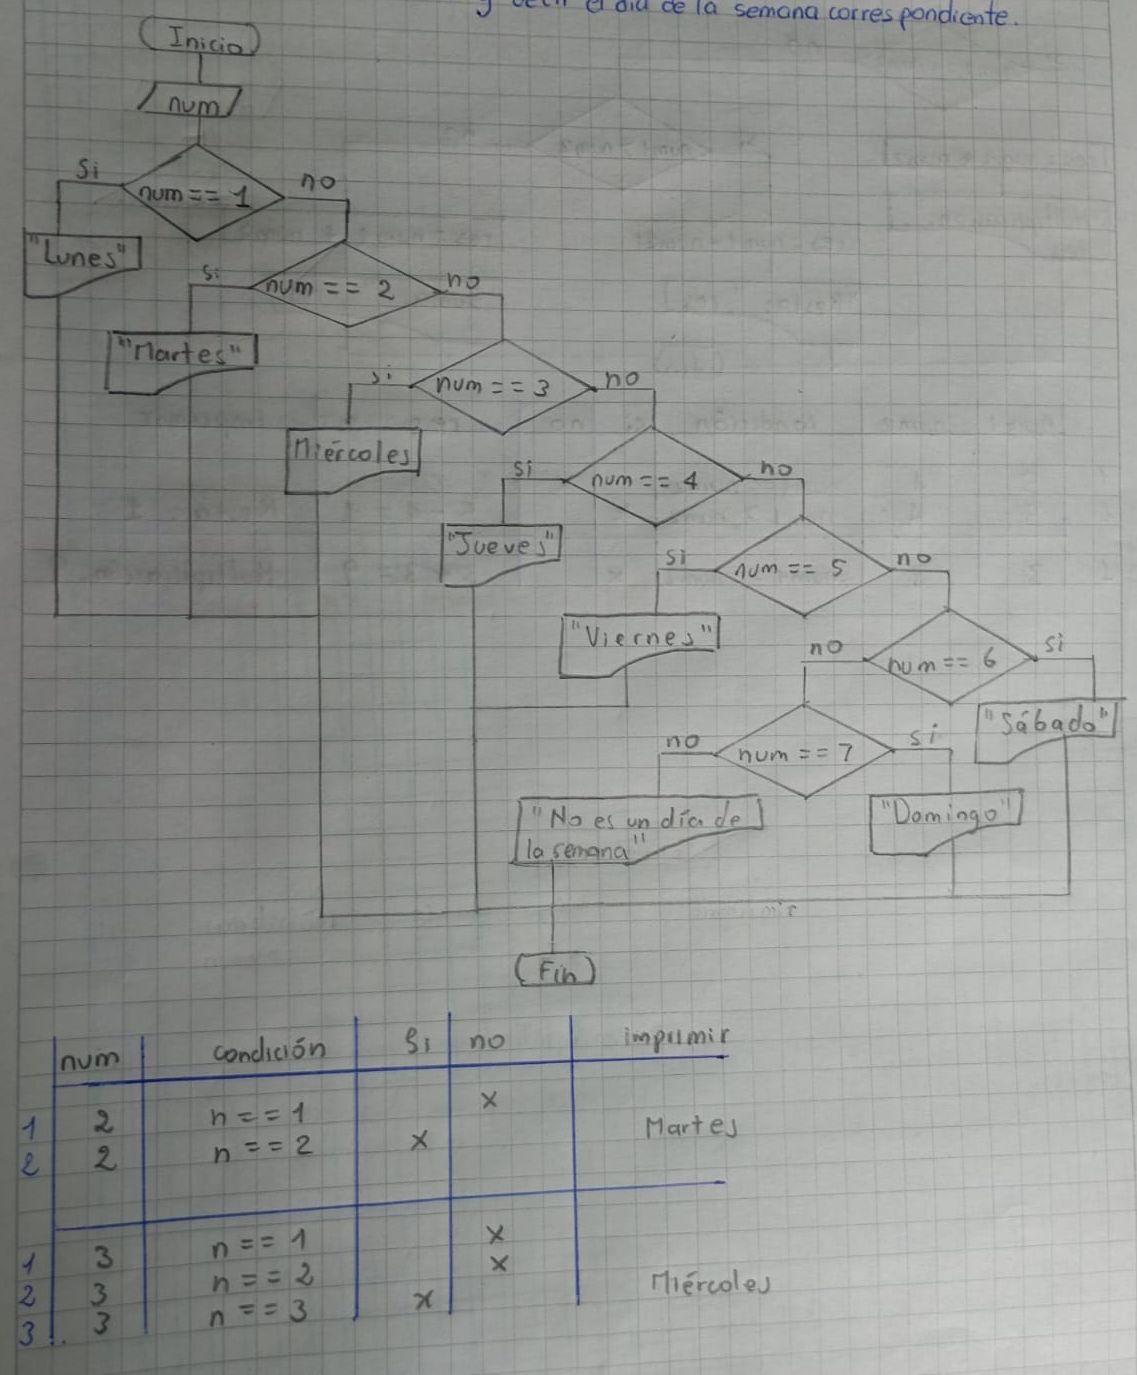
\includegraphics[width=0.9\textwidth]{Img/DF_ej1.jpeg}
                \end{figure}

                \newpage
                \begin{figure}[!h]
                    \centering
                    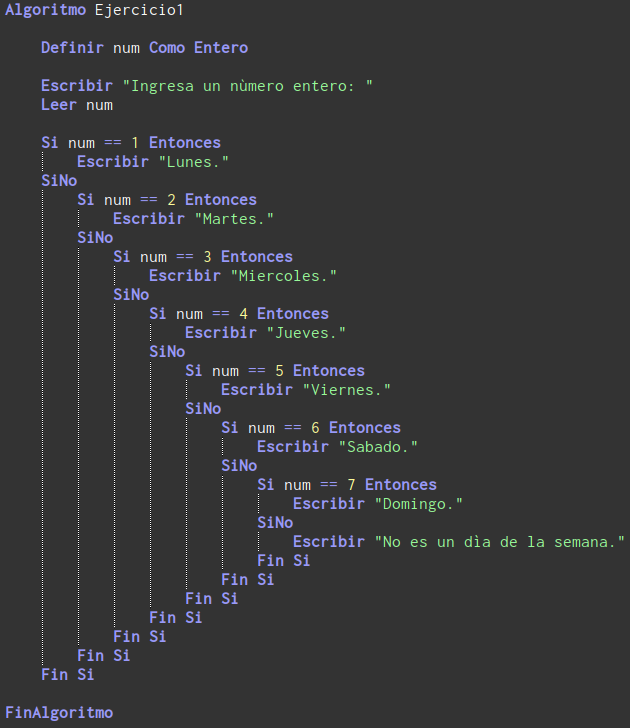
\includegraphics[width=0.6\textwidth]{Img/Cod_ej1.png}
                \end{figure}

                \begin{figure}[!h]
                    \centering
                    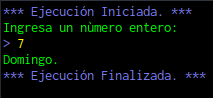
\includegraphics[width=0.4\textwidth]{Img/Ejec_ej1.png}
                \end{figure}

            % Ejercicio 2: -----------------------------------------------
            \newpage
            \item  Leer 2 números; si son iguales que los multiplique, si el primero es mayor que el segundo que los reste y si no que los sume.
            
                \begin{figure}[!h]
                    \centering
                    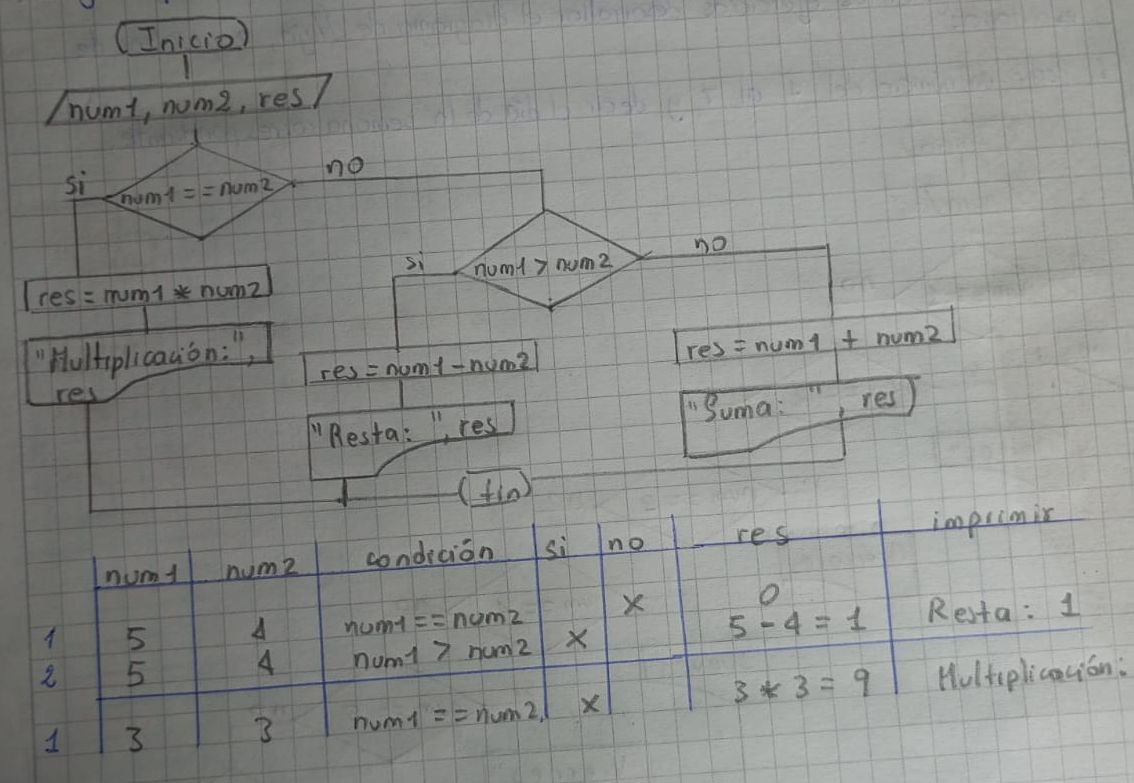
\includegraphics[width=0.9\textwidth]{Img/DF_ej2.jpeg}
                \end{figure}

                \newpage
                \begin{figure}[!h]
                    \centering
                    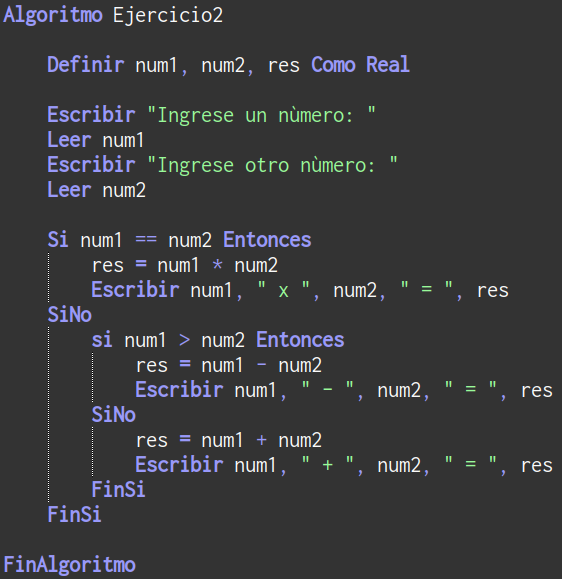
\includegraphics[width=0.7\textwidth]{Img/Cod_ej2.png}
                \end{figure}

                \begin{figure}[!h]
                    \centering
                    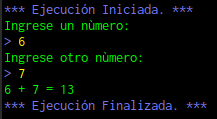
\includegraphics[width=0.4\textwidth]{Img/Ejec_ej2.png}
                \end{figure}

            % Ejercicio 3: -----------------------------------------------
            \newpage
            \item Un hombre desea saber cuánto dinero se genera por concepto de intereses sobre la cantidad que tiene en inversión en el banco. El decidirá reinvertir los intereses siempre y cuando estos excedan a \$7000, y en ese caso desea saber cuánto dinero tendrá finalmente en su cuenta.
            
                \begin{figure}[!h]
                    \centering
                    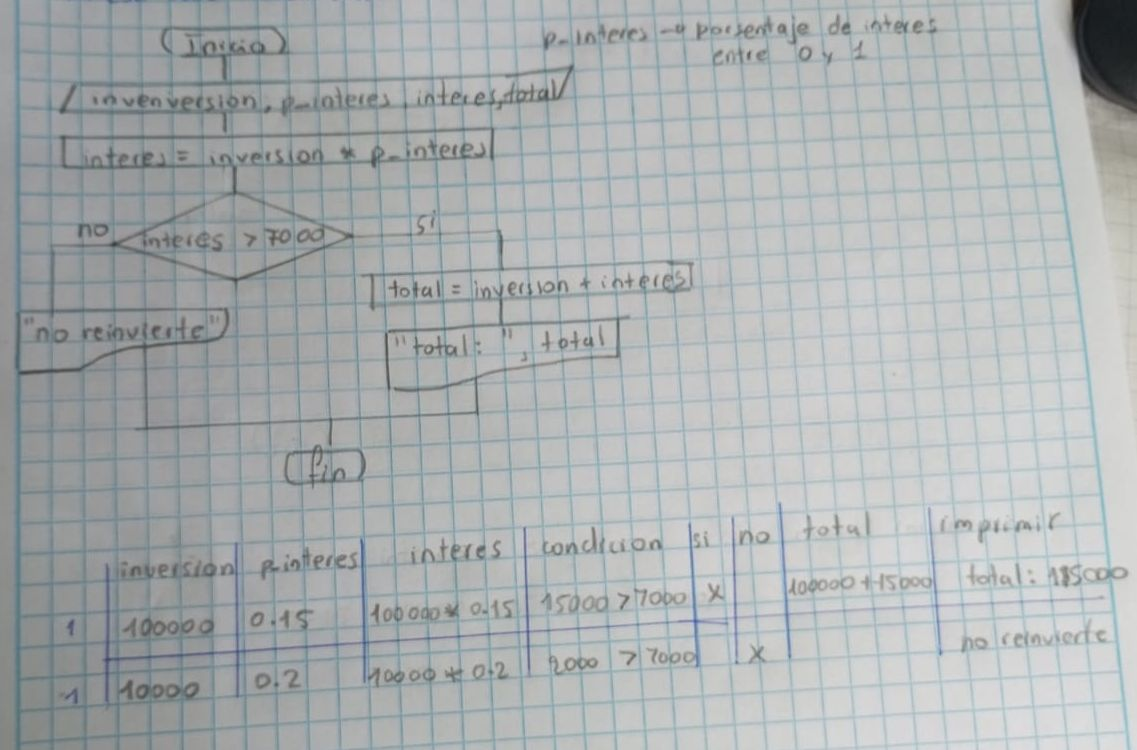
\includegraphics[width=0.9\textwidth]{Img/DF_ej3.jpeg}
                \end{figure}

                \begin{figure}[!h]
                    \centering
                    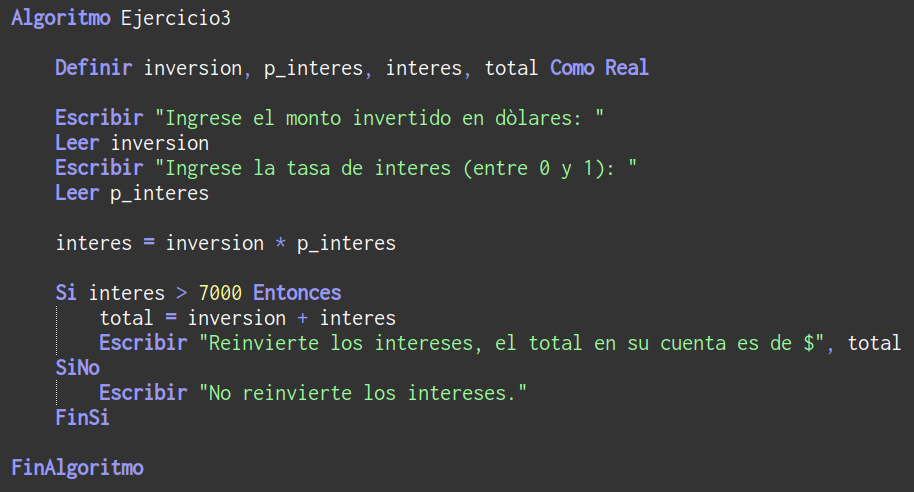
\includegraphics[width=0.7\textwidth]{Img/Cod_ej3.png}
                \end{figure}

                \begin{figure}[!h]
                    \centering
                    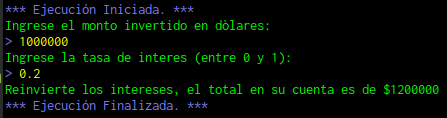
\includegraphics[width=0.5\textwidth]{Img/Ejec_ej3.png}
                \end{figure}
            
            % Ejercicio 4: -----------------------------------------------
            \newpage
            \item Fábricas “El cometa” produce artículos con claves (1, 2, 3, 4, 5 y 6). Se requiere un algoritmo para calcular los precios de venta, para esto hay que considerar lo siguiente: Costo de producción = materia prima + mano de obra + gastos de fabricación. Precio de venta = costo de producción + 45\% de costo de producción. El costo de la mano de obra se obtiene de la siguiente forma: para los productos con clave 3 o 4 se carga 75\% del costo de la materia prima; para los que tienen clave 1 y 5 se carga 80\%, y para los que tienen clave 2 o 6, 85\%. Para calcular el gasto de fabricación se considera que si el artículo que se va a producir tiene claves 2 o 5, este gasto representa 30\% sobre el costo de la materia prima; si las claves son 3 o 6, representa 35 %; si las claves son 1 o 4, representa 28 %. La materia prima tiene el mismo costo para cualquier clave. Represente mediante el diagrama de flujo, el pseudocódigo y el diagrama N/S la solución de este problema. Con las consideraciones anteriores se puede establecer la tabla 3.13 de variables requeridas para el planteamiento del algoritmo correspondiente.
            
                \begin{figure}[!h]
                    \centering
                    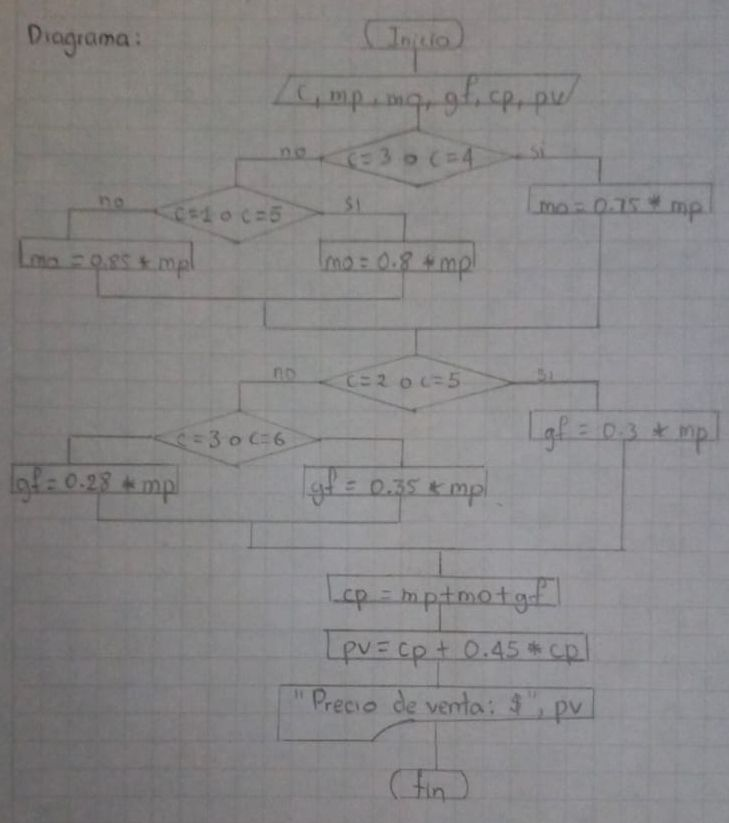
\includegraphics[width=0.7\textwidth]{Img/DF_ej4_1.jpeg}
                \end{figure}

                \newpage
                \begin{figure}[!h]
                    \centering
                    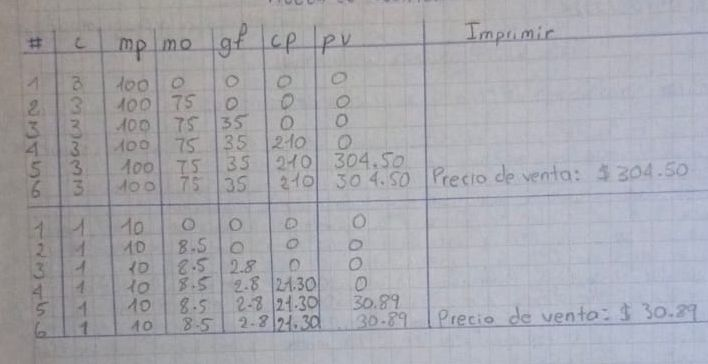
\includegraphics[width=0.6\textwidth]{Img/DF_ej4_2.jpeg}
                \end{figure}

                \begin{figure}[!h]
                    \centering
                    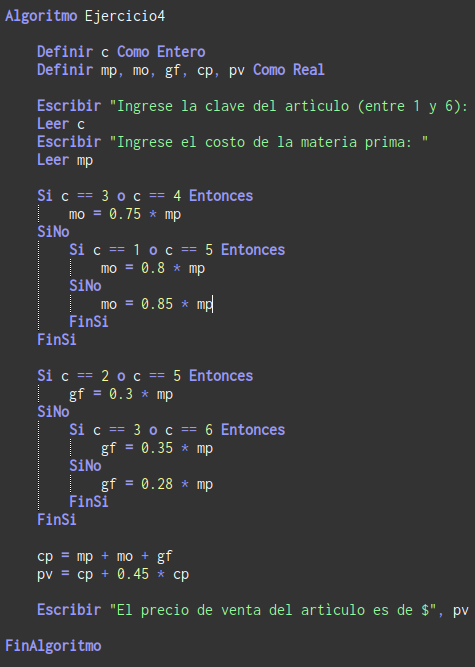
\includegraphics[width=0.6\textwidth]{Img/Cod_ej4.png}
                \end{figure}

                \newpage
                \begin{figure}[!h]
                    \centering
                    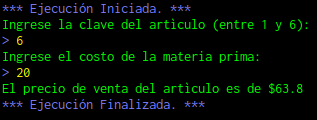
\includegraphics[width=0.5\textwidth]{Img/Ejec_ej4.png}
                \end{figure}
                
            % Ejercicio 5: -----------------------------------------------
            \newpage
            \item Determinar la cantidad de dinero que recibirá un trabajador por concepto de las horas extras trabajadas en una empresa, sabiendo que cuando las horas de trabajo exceden de 40, el resto se consideran horas extras y que  estas se pagan al doble de una hora normal cuando no exceden de 8; si las horas extras exceden de 8 se pagan las primeras 8 al doble de lo que se pagan las horas normales y el resto al triple.
            
                \begin{figure}[!h]
                    \centering
                    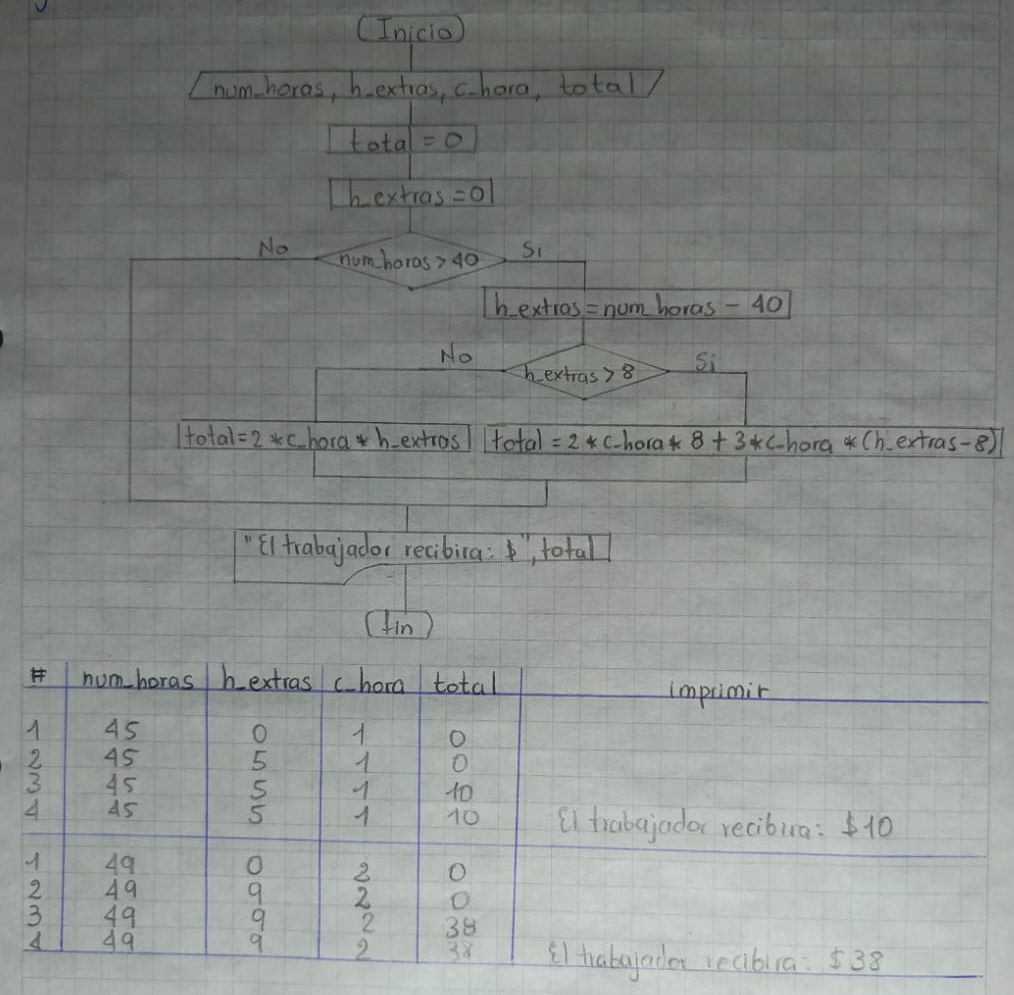
\includegraphics[width=0.9\textwidth]{Img/DF_ej5.jpeg}
                \end{figure}

                \newpage
                \begin{figure}[!h]
                    \centering
                    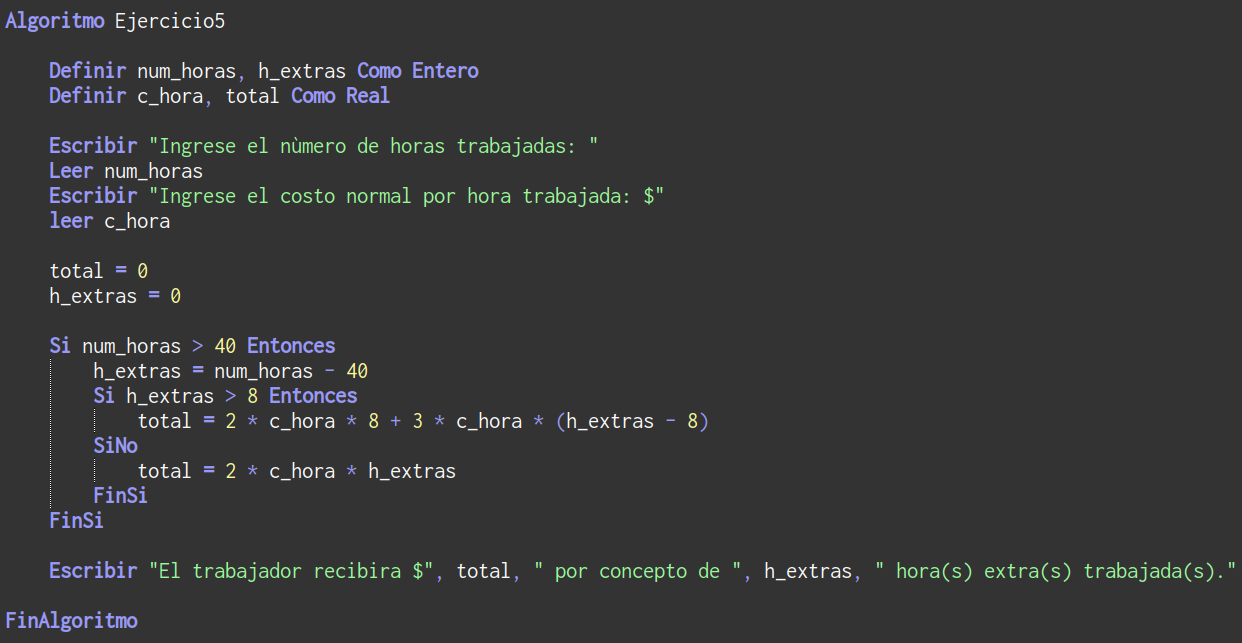
\includegraphics[width=0.9\textwidth]{Img/Cod_ej5.png}
                \end{figure}

                \begin{figure}[!h]
                    \centering
                    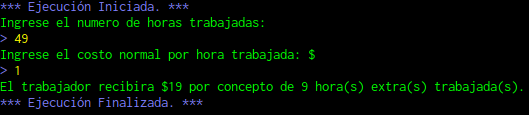
\includegraphics[width=0.7\textwidth]{Img/Ejec_ej5.png}
                \end{figure}
            
            % Ejercicio 6: -----------------------------------------------
            \newpage
            \item Una compañía de seguros para autos ofrece dos tipos de póliza: cobertura amplia (A) y daños a terceros (B). Para el plan A, la cuota base es de \$1,200, y para el B, de \$950. A ambos planes se les carga 10\% del costo si la persona que conduce tiene por hábito beber alcohol, 5\% si utiliza lentes, 5\% si padece alguna enfermedad –como deficiencia cardiaca o diabetes–, y si tiene más de 40 años, se le carga 20\%, de lo contrario sólo 10\%. Todos estos cargos se realizan sobre el costo base. Realice diagrama de flujo y diagrama N/S que represente el algoritmo para determinar cuánto le cuesta a una persona contratar una póliza.
                
                \begin{figure}[!h]
                    \centering
                    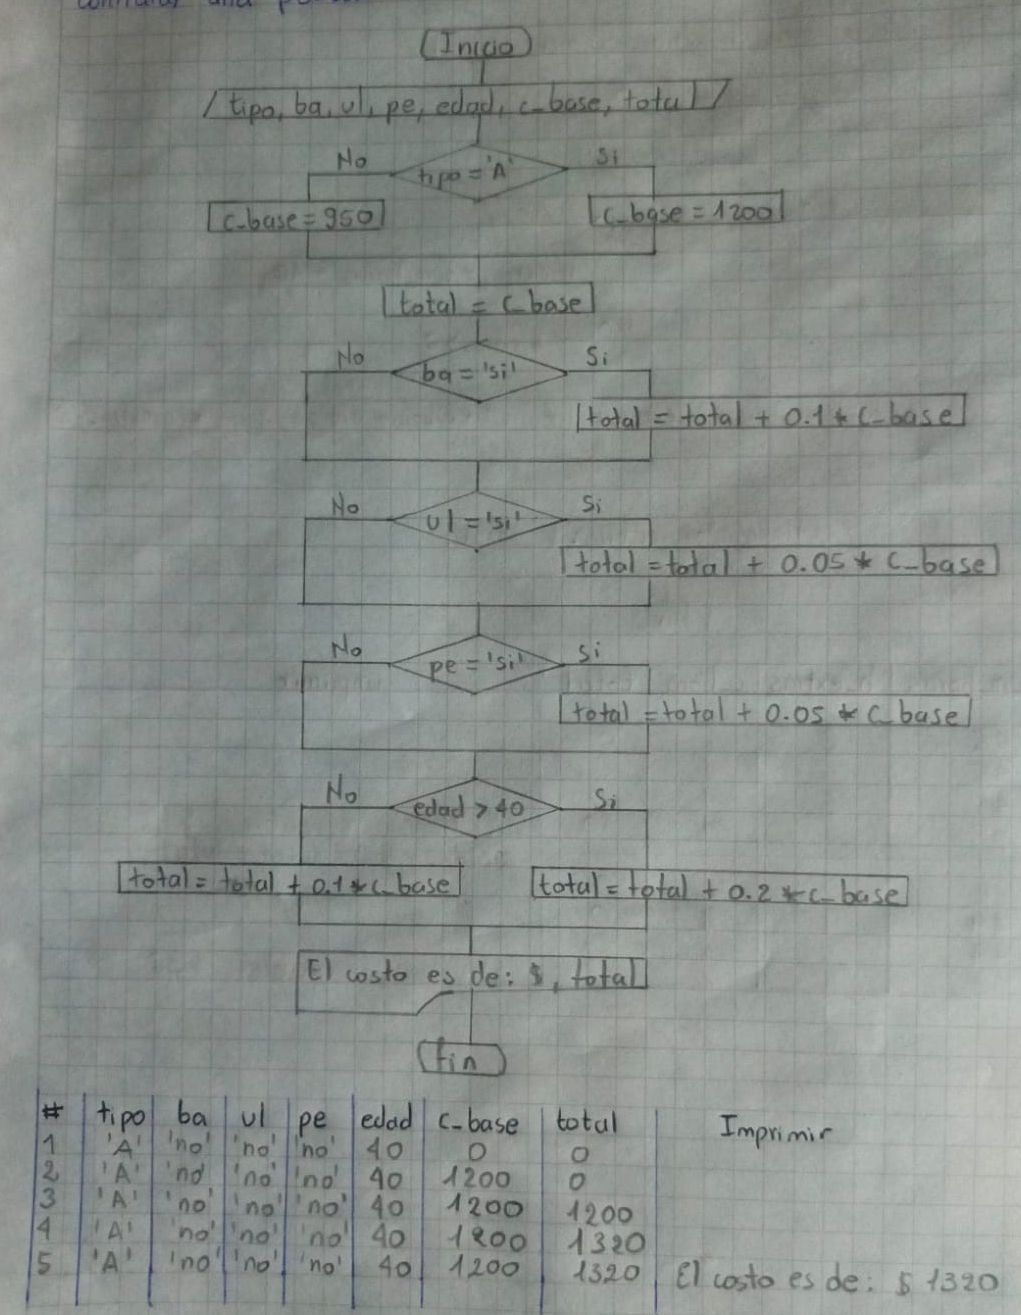
\includegraphics[width=0.7\textwidth]{Img/DF_ej6_1.jpeg}
                \end{figure}

                \newpage
                \begin{figure}[!h]
                    \centering
                    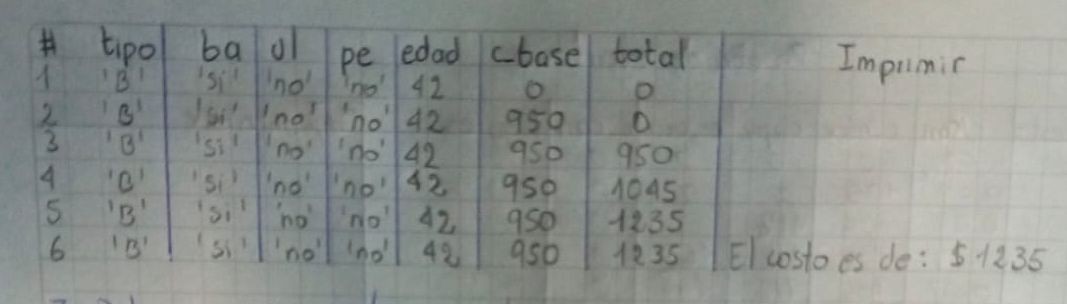
\includegraphics[width=0.9\textwidth]{Img/DF_ej6_2.jpeg}
                \end{figure}

                \begin{figure}[!h]
                    \centering
                    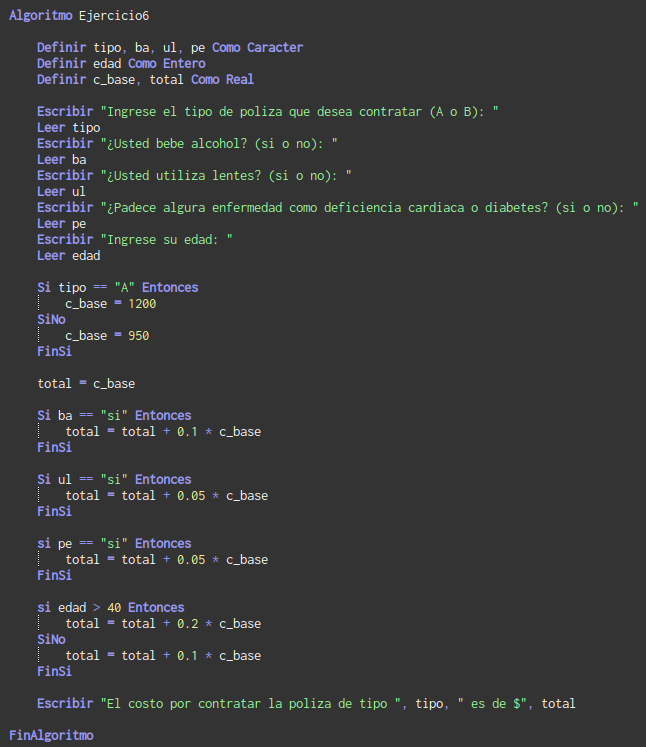
\includegraphics[width=0.8\textwidth]{Img/Cod_ej6.png}
                \end{figure}

                \newpage
                \begin{figure}[!h]
                    \centering
                    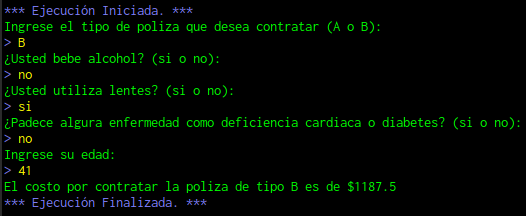
\includegraphics[width=0.7\textwidth]{Img/Ejec_ej6.png}
                \end{figure}
            
            % Ejercicio 7: -----------------------------------------------
            \newpage
            \item Represente un algoritmo mediante un diagrama de flujo para determinar a qué lugar podrá ir de vacaciones una persona, considerando que la línea de autobuses “La tortuga” cobra por kilómetro recorrido. Se debe  considerar el costo del pasaje tanto de ida, como de vuelta; los datos que se conocen y que son fijos son: México, 750 km; P.V., 800 km; Acapulco, 1200 km, y Cancún, 1800 km. También se debe considerar la posibilidad de tener que quedarse en casa.
           
                \begin{figure}[!h]
                    \centering
                    \includegraphics[width=0.9\textwidth]{Img/DF_ej7_1.jpeg}
                \end{figure}

                \newpage
                \begin{figure}[!h]
                    \centering
                    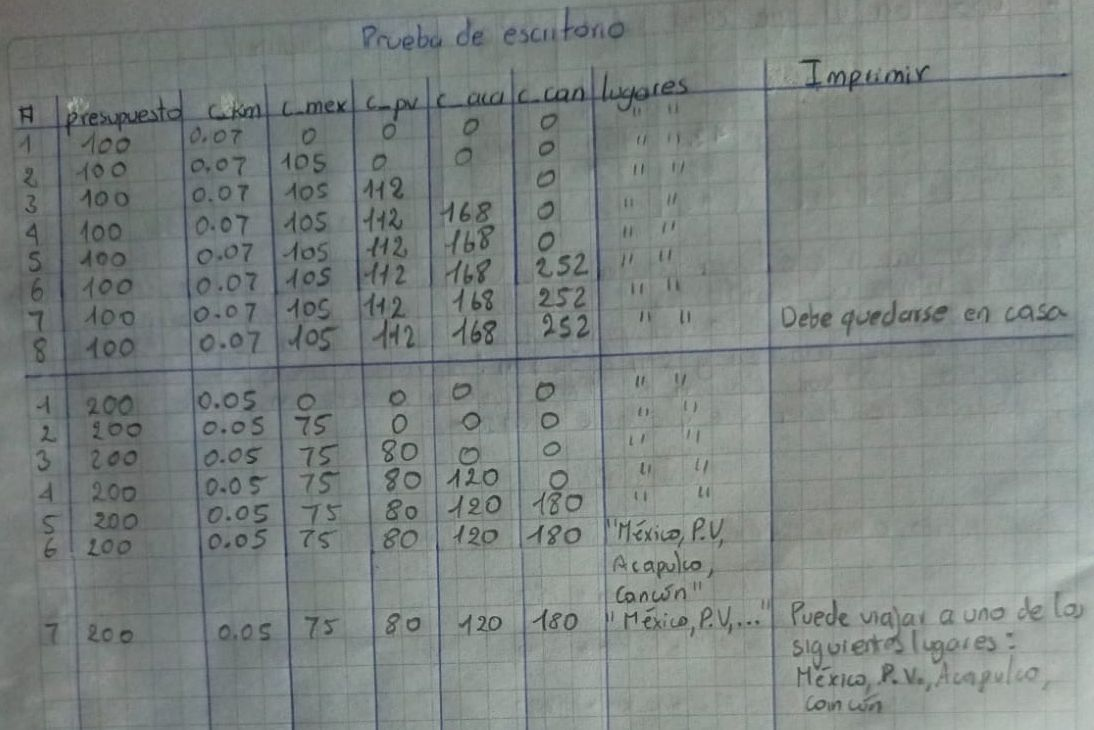
\includegraphics[width=0.8\textwidth]{Img/DF_ej7_2.jpeg}
                \end{figure}

                \begin{figure}[!h]
                    \centering
                    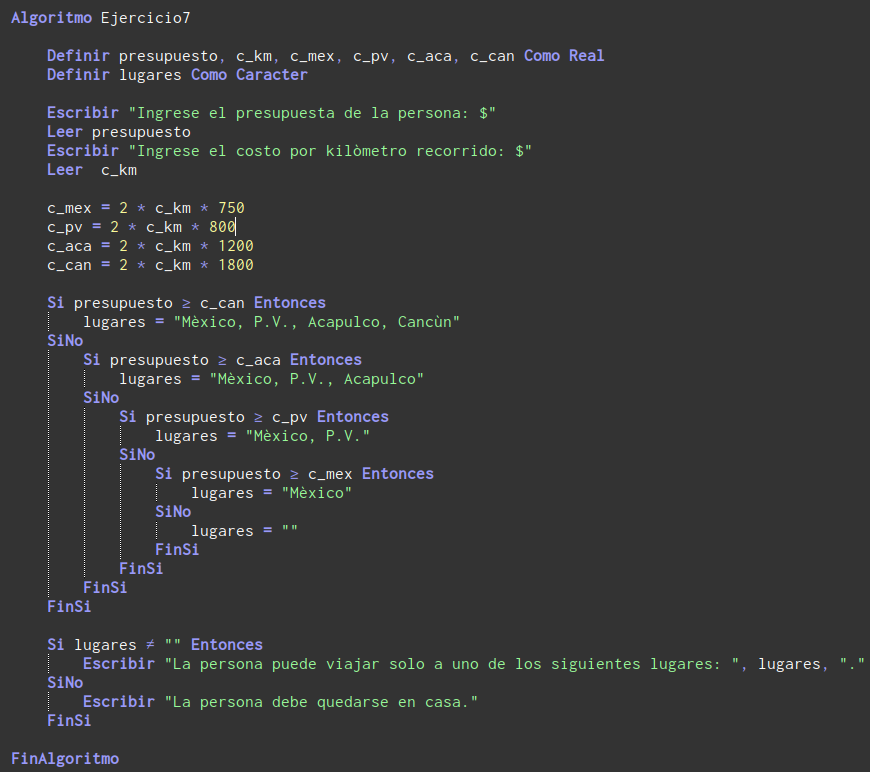
\includegraphics[width=0.8\textwidth]{Img/Cod_ej7.png}
                \end{figure}

                \newpage
                \begin{figure}[!h]
                    \centering
                    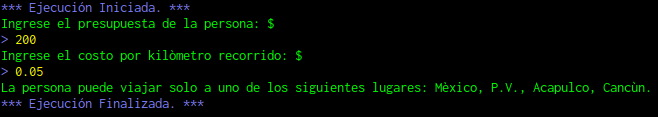
\includegraphics[width=0.8\textwidth]{Img/Ejec_ej7.png}
                \end{figure}
            
            % Ejercicio 8: -----------------------------------------------
            \newpage
            \item Se les dará un bono por antigüedad a los empleados de una tienda. Si tienen un año, se les dará \$100; si tienen 2 años, \$200, y así sucesivamente hasta los 5 años. Para los que tengan más de 5, el bono será de \$1000. Realice un algoritmo y represéntelo mediante el diagrama de flujo, el pseudocódigo y diagrama N/S que permita determinar el bono que recibirá un trabajador.
           
                \begin{figure}[!h]
                    \centering
                    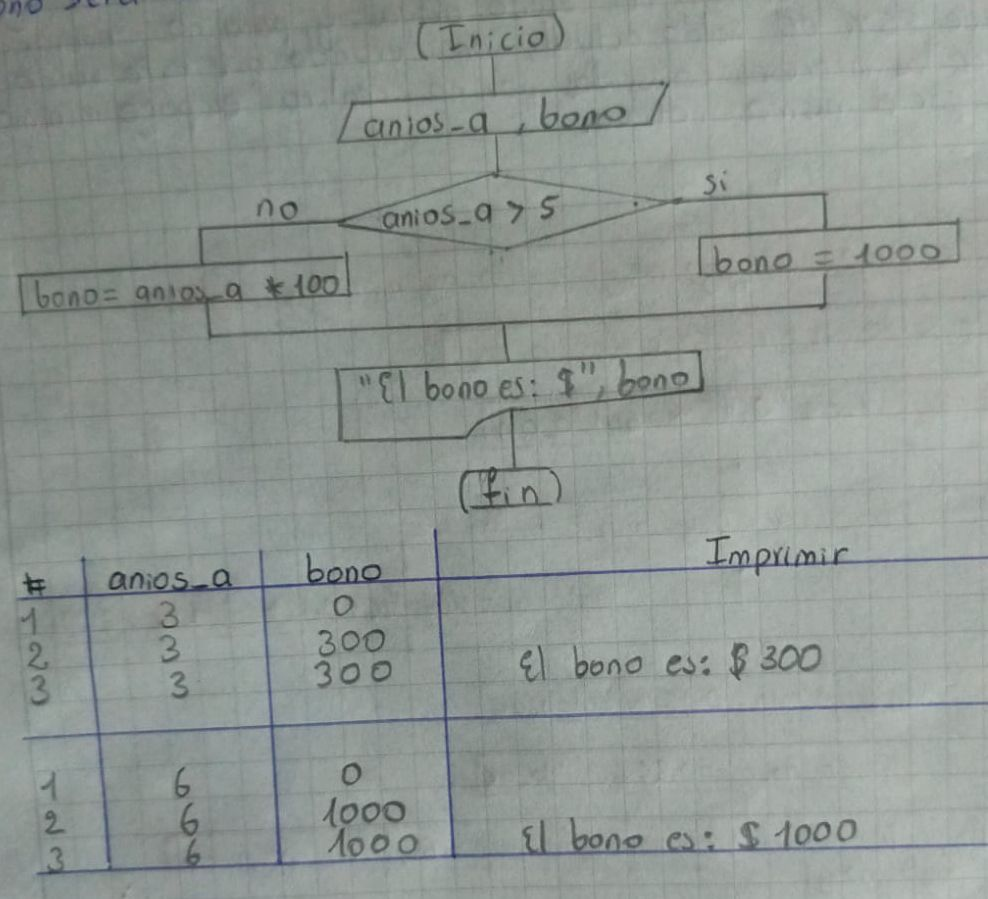
\includegraphics[width=0.9\textwidth]{Img/DF_ej8.jpeg}
                \end{figure}

                \newpage
                \begin{figure}[!h]
                    \centering
                    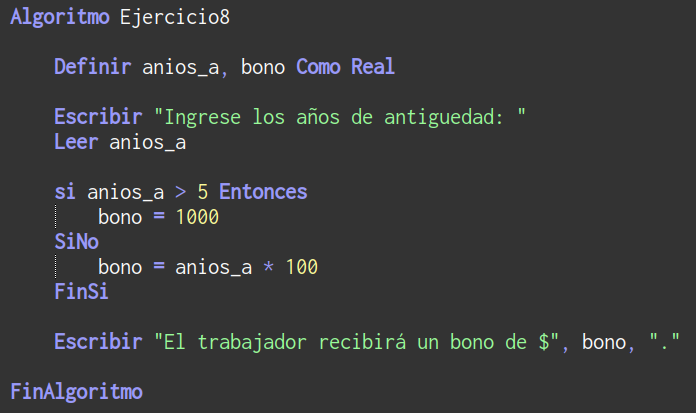
\includegraphics[width=0.8\textwidth]{Img/Cod_ej8.png}
                \end{figure}

                \begin{figure}[!h]
                    \centering
                    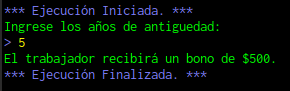
\includegraphics[width=0.6\textwidth]{Img/Ejec_ej8.png}
                \end{figure}
           
            % Ejercicio 9: -----------------------------------------------
            \newpage
            \item El banco “Bandido de peluche” desea calcular para uno de sus clientes el saldo actual, el pago mínimo y el pago para no generar intereses. Los datos que se conocen son: saldo anterior del cliente, monto de las compras que realizó y el pago que depositó en el corte anterior. Para calcular el pago mínimo se debe considerar 15\% del saldo actual, y para no generar intereses corresponde 85\% del saldo actual, considerando que este saldo debe incluir 12\% de los intereses causados por no realizar el pago mínimo y \$200 por multa por el mismo motivo. Realice el algoritmo correspondiente y represéntelo mediante el diagrama de flujo y pseudocódigo.
            
                \begin{figure}[!h]
                    \centering
                    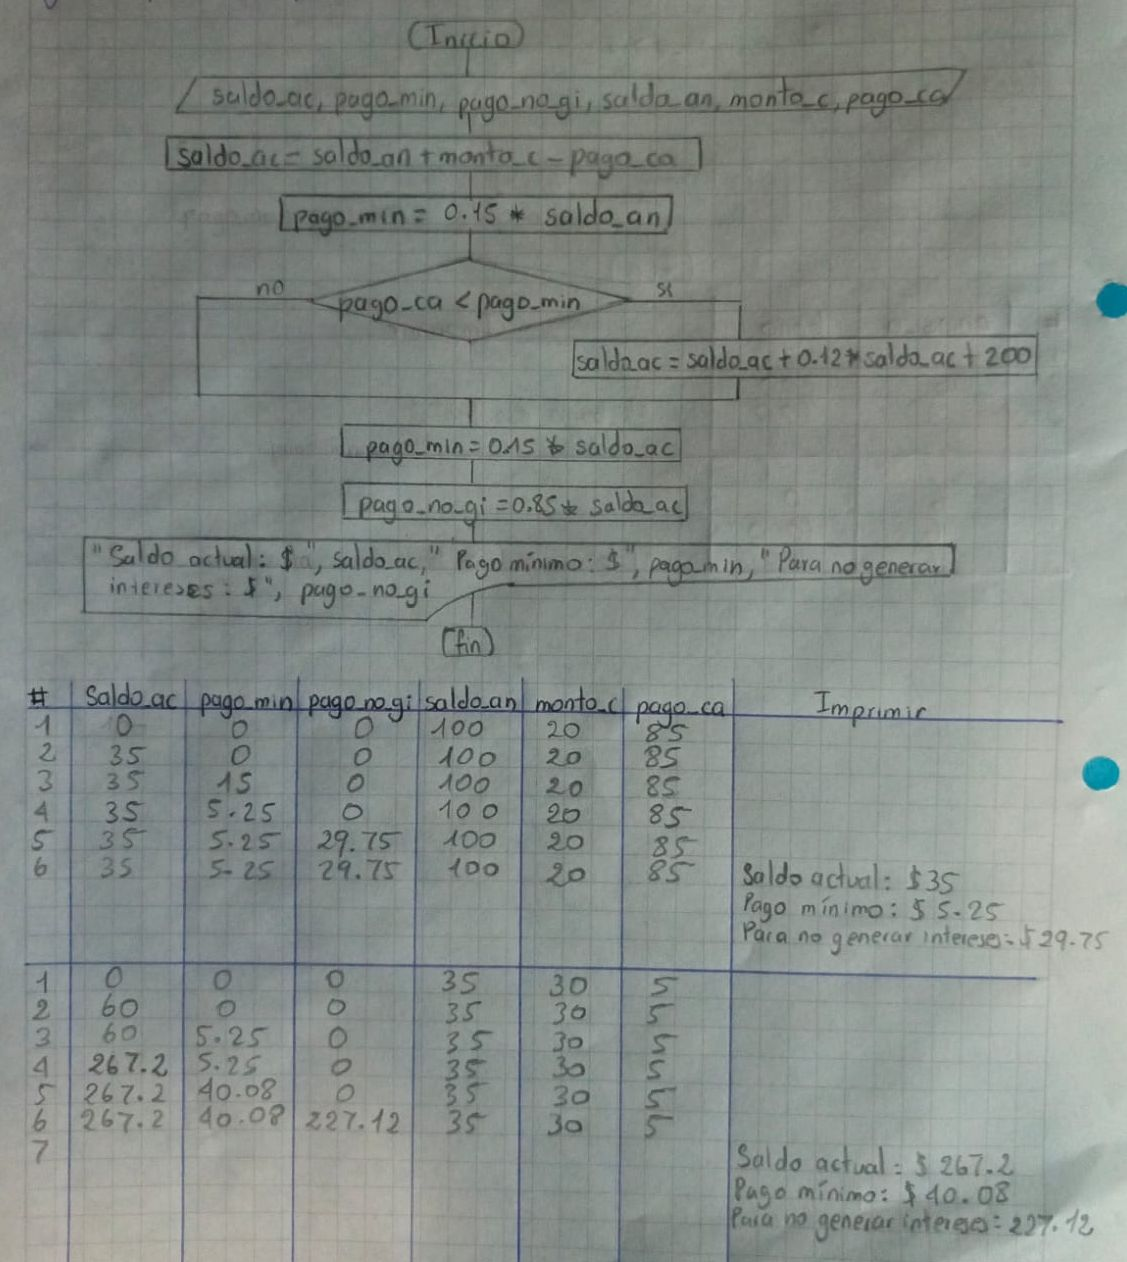
\includegraphics[width=0.9\textwidth]{Img/DF_ej9.jpeg}
                \end{figure}

                \newpage
                \begin{figure}[!h]
                    \centering
                    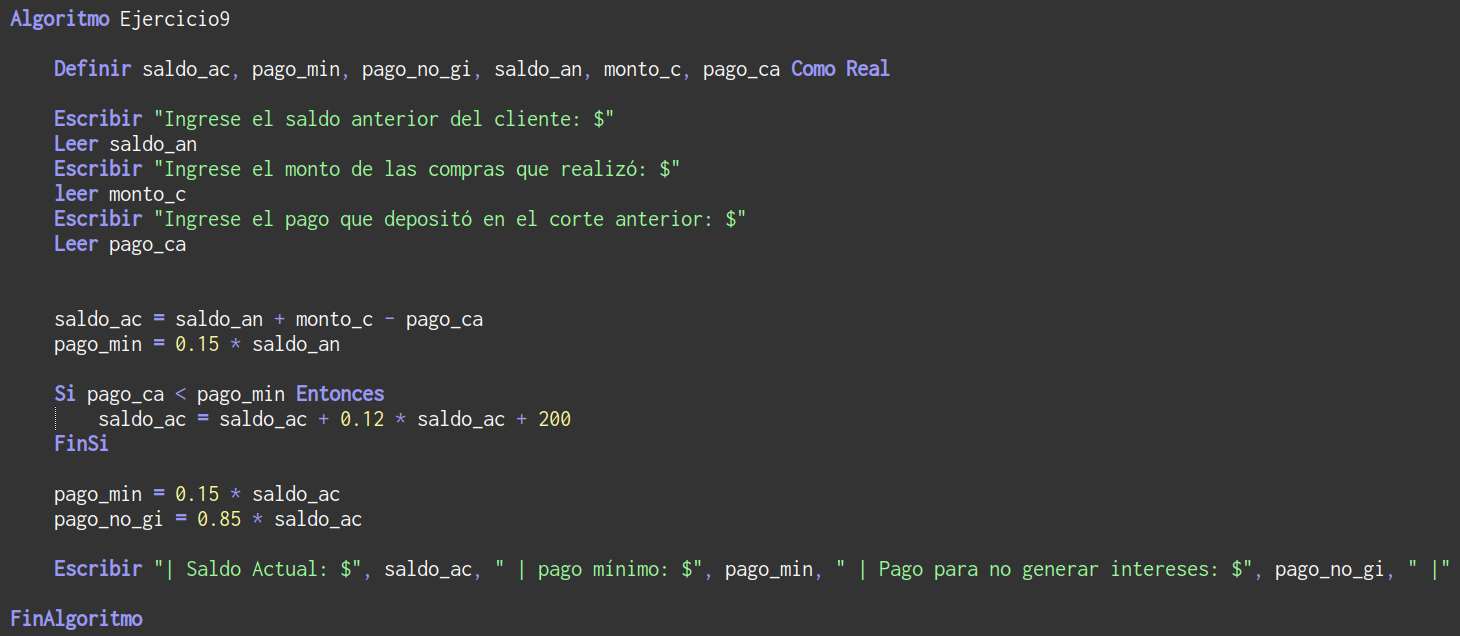
\includegraphics[width=0.9\textwidth]{Img/Cod_ej9.png}
                \end{figure}

                \begin{figure}[!h]
                    \centering
                    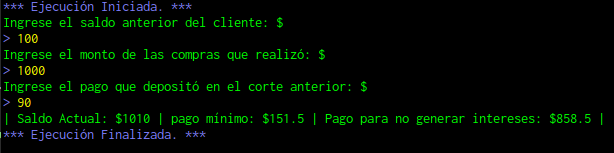
\includegraphics[width=0.8\textwidth]{Img/Ejec_ej9.png}
                \end{figure}
            
            % Ejercicio 10: -----------------------------------------------
            \newpage
            \item Los alumnos de una escuela desean realizar un viaje de estudios, pero requieren determinar cuánto les costará el pasaje, considerando que las tarifas del autobús son las siguientes: si son más de 100 alumnos, el costo es de \$20; si son entre 50 y 100, \$35; entre 20 y 49, \$40, y si son menos de 20 alumnos, \$70 por cada uno. Realice el algoritmo para determinar el costo del pasaje de cada alumno. Represente el algoritmo mediante el diagrama de flujo, el pseudocódigo.
        
                \begin{figure}[!h]
                    \centering
                    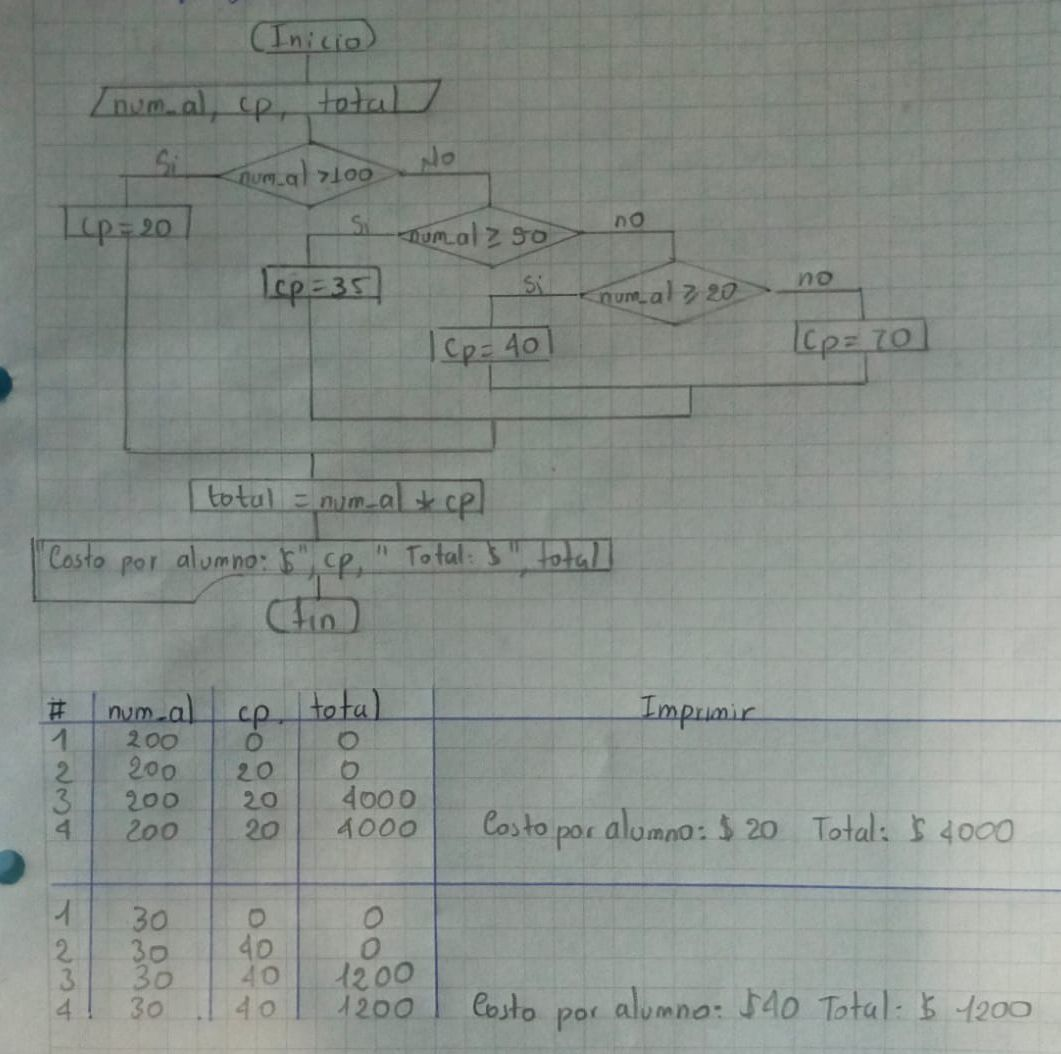
\includegraphics[width=0.9\textwidth]{Img/DF_ej10.jpeg}
                \end{figure}

                \newpage
                \begin{figure}[!h]
                    \centering
                    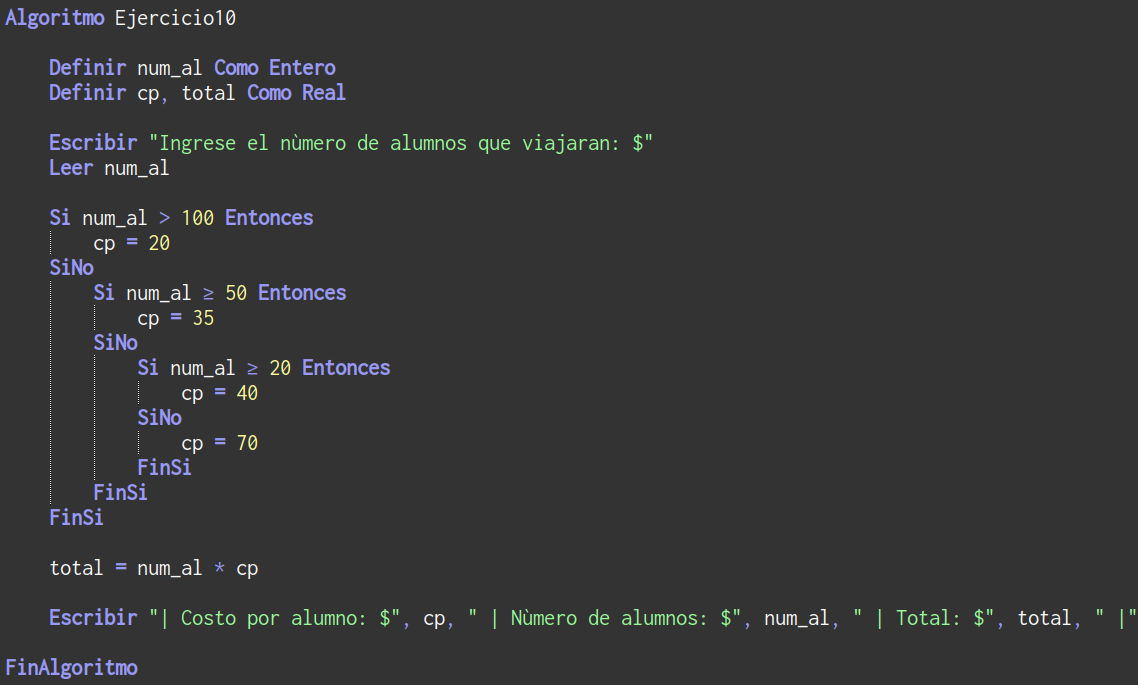
\includegraphics[width=0.9\textwidth]{Img/Cod_ej10.png}
                \end{figure}

                \begin{figure}[!h]
                    \centering
                    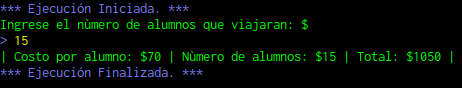
\includegraphics[width=0.7\textwidth]{Img/Ejec_ej10.png}
                \end{figure}
        
        \end{enumerate}

\end{document}